%%%%%%%%%%%%%%%%%%%%%%%%%%%%%%%%%%%%%%%%%%%%%%%%%%%%%%%%%%%%%%%
% P1 Thyroid
% David Miguel Lozano
% Javier Martínez Riberas
% Universidad de Burgos - Septiembre 2016
%%%%%%%%%%%%%%%%%%%%%%%%%%%%%%%%%%%%%%%%%%%%%%%%%%%%%%%%%%%%%%%

% -------------------------------------------------------------
% Preamble
% -------------------------------------------------------------
\documentclass[a4paper,12pt,titlepage]{article}

% -------------------------------------------------------------
% Packages
% -------------------------------------------------------------
\usepackage[utf8]{inputenc}	% Unicode support
\usepackage[T1]{fontenc}		% Font encoding
\usepackage[spanish]{babel}	% Languaje
\usepackage{lmodern}	% Typeface 
\usepackage{textcomp} % Special symbols
\usepackage{graphicx}	% Add pictures
\usepackage{pgfplots} % Graphs and charts
\usepackage{hyperref}	% Add a link to index entries
\usepackage{amsmath}	% Advanced math typesetting
\usepackage{amsfonts}	% Mathematical formulas
\usepackage{amssymb}	% Extended symbol collection
\usepackage{listings}	% Code formatting and highlighting
\usepackage{xcolor}		% Color package
\usepackage{enumitem}	% Customizing lists
\usepackage{parskip}	% Paragraph styles
\usepackage[a4paper]{geometry} 		% Margins
\usepackage[numbers,sort]{natbib}	% Bibliography management 

% -------------------------------------------------------------
% Configuration
% -------------------------------------------------------------
% Images path
\graphicspath{ {img/} }
% Graphs configuration 
\pgfplotsset{width=\textwidth,compat=1.9}
% Hyperlinks coloring
\hypersetup{
	colorlinks,
	linkcolor={green!40!black},
	citecolor={blue!50!black},
	urlcolor={blue!80!black}
}
% Define HRule
\newcommand{\HRule}[1]{\rule{\linewidth}{#1}}

\begin{document}
% -------------------------------------------------------------
% Cover
% -------------------------------------------------------------
\author{David Miguel Lozano \ Javier Martínez Riberas}
\title{P1 Thyroid}
\date{23-09-2016}

\begin{titlepage}
	\centering
	
\includegraphics[width=0.16\textwidth]{ubu-logo.png}\par
	\vspace{0.3cm}
	{\scshape\LARGE Universidad de Burgos \par}
	\vfill
	{\scshape\Large Computación Neuronal y Evolutiva \par}
	\HRule{2pt}
	{\huge\bfseries P1: Thyroid \par}
	\HRule{2pt}
	\\ [0.5cm]
	{Diseñar y entrenar una red neuronal para clasificar pacientes en tres grupos clínicos dependiendo de la patología en la glándula tiroides (pacientes sanos, con hipertiroidismo o con hipertiroidismo).}
	\vfill
	Estudiantes:\par
	{\Large\scshape David Miguel Lozano \\ Javier Martínez Riberas \par}
	\vfill
	Profesor de la asignatura:\par
	\textsc{Álvaro Herrero Cosío}
	\vfill
	{\large 1º semestre 2016 \par}
\end{titlepage}

% -------------------------------------------------------------
% Contents
% -------------------------------------------------------------
\newpage
\tableofcontents
\begin{appendix}
  %\listoffigures
  %\listoftables
\end{appendix}

% -------------------------------------------------------------
% Body
% -------------------------------------------------------------
\newpage

\section{Introduction}

El objetivo de la práctica es diseñar y entrenar una red neuronal para la clasificación de pacientes en tres grupos dependiendo de la patología en la glándula tiroides. Se trata de un problema de reconocimiento de patrones en el que dados unos datos de entrada la red neuronal será capaz de asignarlos a una de las tres clases definidas (pacientes sanos, con hipertiroidismo o con hipertiroidismo). Haremos uso del dataset de ejemplo \emph{Thyroid} que provée Matlab.

Realizaremos un estudio sobre el ajuste en el número de neuronas, ejecutando varios entrenamientos con la red y modificando el valor de este parámetro. Y discutiremos qué configuración nos proporciona los mejores resultados. Por último, explotaremos la red y analizaremos las salidas devueltas.

\section{Motivación}

La motivación que nos llevó a elegir el tema del trabajo fue el que ambos poseíamos algún familiar que sufría alguna alteración en la glándula tiroides. Además, el gran desarrollo que están teniendo las redes neuronales aplicadas a la medicina en los últimos años nos desató interés para adentrarnos en este tema.

\section{Descripción del conjunto de datos}

El conjunto de datos utilizados los hemos obtenido del dataset de ejemplo \emph{Thyroid} que provée Matlab. Los datos provienen del \emph{UCI Machine Learning Repository} \citep{Asuncion+Newman:2007} y fueron donados por la Universidad de California.

El dataset contiene datos de 7200 pacientes agrupados en dos matrices:

\begin{itemize}[noitemsep]
	\item $thyroidInputs$: matriz de 21x7200 con los datos de los 7200 pacientes caracterizados por 15 atributos binarios y 6 atributos continuos.
	\item $thyroidTargets$: matriz de 3x7200 en donde se asocia un vector de tres clases a cada paciente. En este vector se define a cuál de las tres clases pertenece el paciente.
\end{itemize}

\newpage

Las tres clases que contiene el dataset son:

\begin{enumerate}[noitemsep]
	\item Paciente sano.
	\item Paciente con hipertiroidismo.
	\item Paciente con hipotiroidismo.
\end{enumerate}

La descripción precisa del significado real de cada atributo y los valores que puede tomar la podemos encontrar en la página web del repositorio \citep{Asuncion+Newman:2007}. Para nuestra tarea no nos es relevante.

Nuestro objetivo es construir una red neuronal y entrenarla con los datos reales propocionados para que posteriormente sea capaz de clasificar a nueveos pacientes. 

Dividiremos aleatoriamente los datos que contiene el data set en tres grupos:

\begin{itemize}[noitemsep]
	\item $Training (70\%)$: lo utilizaremos para el entrenamiento supervisado.
	\item $Validation (15\%)$: lo utilizaremos para comprobar cuándo la red está generalizando y detener el entranamiento para evitar el sobreajuste (\textit{overfitting}).
	\item $Test (15\%)$: lo utilizaremos de forma totalmente independiente al entrenamiento para comprobar la generalización de la red.
\end{itemize}

\section{Descripción del procedimiento}

Para resolver la tarea planteada creamos una red neuronal con una topología \href{http://www.mathworks.com/help/nnet/ref/patternnet.html}{patternnet}. Esta topología posée dos capas \textit{feedforward}, con una función de activación sigmoidal en la capa oculta y una función \textit{softmax} en la capa de salida. Se caracteriza por poder clasificar vectores con una precisión arbitrariamente buena si posée suficientes neuronas en su capa oculta.

\begin{figure}[!ht]
	\centering
	\label{fig:patternnet}
	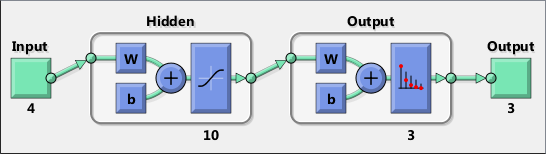
\includegraphics[width=\textwidth]{patternnet.png}
	\caption{Pattern recognition network.}
\end{figure}

En nuestro estudio vamos a variar el número de neuronas de la capa oculta para intentar conseguir los mejores resultados (tanto en error, como en tiempo de entrenamiento). La capa de salida siempre va a tener tres neuronas, cada una se encargará de evaluar la pertenercia a una de las tres clases.

Otro elemento que puede afectar al rendimiento de nuestra red es la función de entrenamiento utilizada. Probaremos ocho funciones distintas que implementa Matlab para comparar resultados.

Para realizar el estudio lo más automatizado posible, hemos creado una función ($autoTrain$) que se encarga de entrenar la red de acuerdo con los parámetros pasados. Por otro lado tenemos un script ($trainAndShow.m$) que llama a esta función variando el número de neuronas de la capa oculta (de 1 a 100 con paso 1) y los algoritmos de entrenamiento ($trainbfg$, $trainrp$, $trainscg$, $traincgb$,  $traincgf$, $traincgp$, $trainoss$ y $traingdx$). Además, repite el entrenamiento de cada caso 10 veces para disminuir la varianza y la aleatoriedad.

El script proporciona como salida el valor de confusión medio en cada caso,  la matríz de confusión completa y el tiempo medio de entrenamiento. Con tres formatos de salida, un primer formato legible para humanos, otro formateado para la librería de gráficos \textit{pgfplots} y un tercer formato como CSV.

\emph{*Todo el código generado en esta práctica se encuentra disponible en el siguiente repositorio: 
\href{https://github.com/davidmigloz/neuronal-networks/tree/master/P1\_Thyroid}{P1\_Thyroid}.}

\section{Estudio}

asdfasdf

\newpage
\newgeometry{top=1cm,bottom=2.5cm}

\begin{tikzpicture}[every plot/.append style={semithick}]
\begin{axis}[
    title={Evolución del valor de confusión},
    xlabel={Número de neuronas en la capa oculta},
    ylabel={Valor de confusión},
    xmin=1, xmax=50,
    ymin=0.03, ymax=0.08,
    xtick={1,10,20,30,40,50},
    ytick={0.03,0.04,0.05,0.06,0.07,0.08},
    legend pos=north east,
    ymajorgrids=true,
    grid style=dashed,
    scaled ticks=false, % prevent scale labels
    tick label style={/pgf/number format/fixed}, % label number format
]

\addplot
    coordinates {
(1,0.074167)(2,0.067764)(3,0.072556)(4,0.059986)(5,0.057514)(6,0.062403)(7,0.056681)(8,0.047250)(9,0.051042)(10,0.052542)(11,0.045278)(12,0.054181)(13,0.053569)(14,0.042542)(15,0.055014)(16,0.049542)(17,0.055556)(18,0.052361)(19,0.053528)(20,0.048111)(21,0.051292)(22,0.045903)(23,0.050306)(24,0.050194)(25,0.053056)(26,0.046681)(27,0.053514)(28,0.051917)(29,0.055444)(30,0.048000)(31,0.051528)(32,0.058431)(33,0.053972)(34,0.050458)(35,0.047583)(36,0.047458)(37,0.047056)(38,0.056722)(39,0.053889)(40,0.056097)(41,0.049056)(42,0.041597)(43,0.056153)(44,0.039375)(45,0.050208)(46,0.046194)(47,0.041042)(48,0.050111)(49,0.052472)(50,0.050347)
    };
    \addlegendentry{trainbfg}
    
\addplot
    coordinates {
(1,0.074181)(2,0.070847)(3,0.063333)(4,0.060000)(5,0.056931)(6,0.056750)(7,0.057264)(8,0.055611)(9,0.056000)(10,0.056083)(11,0.056458)(12,0.056667)(13,0.056736)(14,0.057472)(15,0.055014)(16,0.057139)(17,0.057514)(18,0.057986)(19,0.056403)(20,0.054583)(21,0.057986)(22,0.056278)(23,0.054333)(24,0.055347)(25,0.055389)(26,0.055708)(27,0.053361)(28,0.056000)(29,0.054486)(30,0.054806)(31,0.056333)(32,0.054403)(33,0.053264)(34,0.054028)(35,0.055625)(36,0.053056)(37,0.052972)(38,0.054472)(39,0.055292)(40,0.055917)(41,0.057125)(42,0.056583)(43,0.056417)(44,0.055194)(45,0.055458)(46,0.054111)(47,0.053250)(48,0.056083)(49,0.054125)(50,0.055806)
    };
    \addlegendentry{trainrp}

\addplot
    coordinates {
(1,0.063875)(2,0.065778)(3,0.058097)(4,0.060972)(5,0.059389)(6,0.057083)(7,0.054361)(8,0.056097)(9,0.056750)(10,0.055972)(11,0.057208)(12,0.056389)(13,0.057861)(14,0.055403)(15,0.059819)(16,0.056153)(17,0.058431)(18,0.056194)(19,0.057917)(20,0.055889)(21,0.056556)(22,0.057375)(23,0.054333)(24,0.054028)(25,0.059292)(26,0.054653)(27,0.055458)(28,0.056833)(29,0.056181)(30,0.057194)(31,0.056403)(32,0.057361)(33,0.055264)(34,0.055569)(35,0.059319)(36,0.057319)(37,0.055694)(38,0.055597)(39,0.054681)(40,0.055653)(41,0.053611)(42,0.056278)(43,0.056875)(44,0.056333)(45,0.056903)(46,0.056347)(47,0.058278)(48,0.056514)(49,0.059444)(50,0.058486)
    };
    \addlegendentry{trainscg}

\addplot
    coordinates {
(1,0.068264)(2,0.063472)(3,0.057083)(4,0.055625)(5,0.047528)(6,0.052111)(7,0.041444)(8,0.043597)(9,0.052389)(10,0.052708)(11,0.037736)(12,0.053139)(13,0.051111)(14,0.039222)(15,0.048972)(16,0.041750)(17,0.049681)(18,0.048569)(19,0.050389)(20,0.042944)(21,0.042167)(22,0.052944)(23,0.050875)(24,0.054625)(25,0.051889)(26,0.055792)(27,0.043736)(28,0.046569)(29,0.047069)(30,0.052639)(31,0.046028)(32,0.049569)(33,0.047792)(34,0.050792)(35,0.047417)(36,0.044194)(37,0.050417)(38,0.048458)(39,0.045444)(40,0.045958)(41,0.048083)(42,0.052958)(43,0.042139)(44,0.054986)(45,0.055375)(46,0.042139)(47,0.046931)(48,0.054139)(49,0.049958)(50,0.049264)
    };
    \addlegendentry{traincgb}
                    
\end{axis}
\end{tikzpicture}

\begin{tikzpicture}[every plot/.append style={semithick}]
\begin{axis}[
    xlabel={Número de neuronas en la capa oculta},
    ylabel={Valor de confusión},
    xmin=1, xmax=50,
    ymin=0.035, ymax=0.08,
    xtick={1,10,20,30,40,50},
    ytick={0.03,0.04,0.05,0.06,0.07,0.08},
    legend pos=south east,
    ymajorgrids=true,
    grid style=dashed,
    scaled ticks=false, % prevent scale labels
    tick label style={/pgf/number format/fixed}, % label number format
]

\addplot
    coordinates {
(1,0.074139)(2,0.072153)(3,0.072778)(4,0.069181)(5,0.067347)(6,0.065806)(7,0.064931)(8,0.061042)(9,0.057458)(10,0.063597)(11,0.056097)(12,0.059361)(13,0.061944)(14,0.057792)(15,0.059236)(16,0.057292)(17,0.053972)(18,0.053472)(19,0.058014)(20,0.053375)(21,0.052181)(22,0.054917)(23,0.052556)(24,0.051194)(25,0.050653)(26,0.055250)(27,0.055931)(28,0.055069)(29,0.051500)(30,0.056306)(31,0.051736)(32,0.053042)(33,0.052792)(34,0.052500)(35,0.048514)(36,0.051083)(37,0.054625)(38,0.050236)(39,0.044972)(40,0.050875)(41,0.053472)(42,0.053611)(43,0.045056)(44,0.048708)(45,0.050583)(46,0.044375)(47,0.047903)(48,0.049319)(49,0.051167)(50,0.051181)
    };
    \addlegendentry{traincgf}

\addplot
    coordinates {
(1,0.070389)(2,0.067708)(3,0.059181)(4,0.060194)(5,0.055764)(6,0.057319)(7,0.055597)(8,0.055903)(9,0.055014)(10,0.056458)(11,0.057292)(12,0.053292)(13,0.055042)(14,0.052236)(15,0.055306)(16,0.057292)(17,0.053208)(18,0.053736)(19,0.057653)(20,0.049958)(21,0.056917)(22,0.057708)(23,0.054375)(24,0.055125)(25,0.057097)(26,0.057014)(27,0.056083)(28,0.053764)(29,0.056694)(30,0.052292)(31,0.057222)(32,0.051361)(33,0.054917)(34,0.054111)(35,0.055319)(36,0.050361)(37,0.053625)(38,0.054431)(39,0.055361)(40,0.052903)(41,0.052972)(42,0.055028)(43,0.050861)(44,0.051958)(45,0.054861)(46,0.057944)(47,0.054361)(48,0.058597)(49,0.052514)(50,0.056875)
    };
    \addlegendentry{traincgp}
    
\addplot
    coordinates {
(1,0.070778)(2,0.067583)(3,0.067639)(4,0.057319)(5,0.062194)(6,0.057194)(7,0.064000)(8,0.057708)(9,0.054972)(10,0.059250)(11,0.054778)(12,0.057083)(13,0.056639)(14,0.058875)(15,0.056736)(16,0.055708)(17,0.054681)(18,0.054069)(19,0.057181)(20,0.056542)(21,0.057153)(22,0.053306)(23,0.056556)(24,0.058861)(25,0.057556)(26,0.056264)(27,0.057014)(28,0.057736)(29,0.056639)(30,0.056792)(31,0.057000)(32,0.056375)(33,0.057361)(34,0.057222)(35,0.055375)(36,0.057250)(37,0.058861)(38,0.056028)(39,0.055319)(40,0.053125)(41,0.055181)(42,0.056861)(43,0.056931)(44,0.055986)(45,0.055903)(46,0.057708)(47,0.056708)(48,0.057236)(49,0.056292)(50,0.057097)
    };
    \addlegendentry{trainoss}
    
\addplot
    coordinates {
(1,0.074167)(2,0.073556)(3,0.070833)(4,0.071528)(5,0.069014)(6,0.069917)(7,0.069903)(8,0.069375)(9,0.067472)(10,0.067264)(11,0.067181)(12,0.065806)(13,0.069958)(14,0.066528)(15,0.067736)(16,0.064764)(17,0.069250)(18,0.068111)(19,0.065111)(20,0.065056)(21,0.067000)(22,0.067611)(23,0.066250)(24,0.066000)(25,0.067931)(26,0.068875)(27,0.068139)(28,0.064514)(29,0.067931)(30,0.066625)(31,0.069069)(32,0.068611)(33,0.069319)(34,0.066792)(35,0.078778)(36,0.067764)(37,0.077833)(38,0.071222)(39,0.078681)(40,0.064389)(41,0.072486)(42,0.069694)(43,0.069694)(44,0.076792)(45,0.077736)(46,0.083389)(47,0.078472)(48,0.067000)(49,0.073889)(50,0.069681)
    };
    \addlegendentry{traingdx}      
                        
\end{axis}
\end{tikzpicture}

\newpage

\begin{tikzpicture}[every plot/.append style={semithick}]
\begin{axis}[
    title={Evolución del tiempo de entrenamiento},
    xlabel={Número de neuronas en la capa oculta},
    ylabel={Tiempo (s)},
    xmin=1, xmax=50,
    ymin=0, ymax=5,
    xtick={1,10,20,30,40,50},
    legend pos=north east,
    ymajorgrids=true,
    grid style=dashed,
    scaled ticks=false, % prevent scale labels
    tick label style={/pgf/number format/fixed}, % label number format
]

\addplot
    coordinates {
(1,0.801562)(2,0.773438)(3,0.879687)(4,1.398438)(5,2.479687)(6,1.701563)(7,2.498438)(8,3.678125)(9,4.343750)(10,4.023438)(11,5.843750)(12,5.215625)(13,5.926563)(14,8.187500)(15,6.839062)(16,9.581250)(17,9.698438)(18,11.779688)(19,11.412500)(20,14.092188)(21,13.120313)(22,20.200000)(23,18.621875)(24,21.139063)(25,19.675000)(26,23.539063)(27,20.375000)(28,25.926562)(29,24.084375)(30,32.139063)(31,27.175000)(32,23.542188)(33,26.528125)(34,35.023438)(35,42.085938)(36,47.539063)(37,48.171875)(38,40.892187)(39,50.700000)(40,53.690625)(41,69.996875)(42,86.618750)(43,60.521875)(44,129.239062)(45,90.700000)(46,129.045312)(47,143.954688)(48,126.051563)(49,121.410938)(50,127.959375)
    };
    \addlegendentry{trainbfg}
    
\addplot
    coordinates {
(1,0.329688)(2,0.351563)(3,0.628125)(4,0.592187)(5,0.707812)(6,0.778125)(7,0.700000)(8,0.676562)(9,0.767188)(10,0.748437)(11,0.825000)(12,0.803125)(13,0.814063)(14,0.703125)(15,0.890625)(16,0.831250)(17,0.756250)(18,0.700000)(19,0.901563)(20,0.984375)(21,0.746875)(22,0.828125)(23,1.146875)(24,0.912500)(25,0.971875)(26,0.950000)(27,1.126562)(28,0.851563)(29,1.015625)(30,1.064062)(31,0.967187)(32,1.065625)(33,1.168750)(34,1.160938)(35,1.134375)(36,1.087500)(37,1.125000)(38,1.139063)(39,0.984375)(40,1.028125)(41,0.910937)(42,0.946875)(43,1.007813)(44,1.143750)(45,1.193750)(46,1.290625)(47,1.482813)(48,1.103125)(49,1.267187)(50,1.156250)
    };
    \addlegendentry{trainrp}

\addplot
    coordinates {
(1,0.514062)(2,0.523438)(3,0.721875)(4,0.731250)(5,0.721875)(6,0.801562)(7,0.982812)(8,0.837500)(9,0.823438)(10,0.920312)(11,0.925000)(12,1.032812)(13,0.835938)(14,0.970313)(15,1.203125)(16,1.042188)(17,0.920312)(18,1.151563)(19,1.056250)(20,1.134375)(21,1.248438)(22,1.143750)(23,1.426563)(24,1.426563)(25,1.057813)(26,1.396875)(27,1.564062)(28,1.276563)(29,1.425000)(30,1.307813)(31,1.296875)(32,1.298437)(33,1.700000)(34,1.448438)(35,1.175000)(36,1.351563)(37,1.465625)(38,1.707813)(39,1.817188)(40,1.532812)(41,1.860937)(42,3.260937)(43,1.542188)(44,1.526563)(45,1.589063)(46,3.514063)(47,1.571875)(48,1.565625)(49,3.379688)(50,1.515625)
    };
    \addlegendentry{trainscg}

\addplot
    coordinates {
(1,0.523438)(2,0.765625)(3,1.375000)(4,1.254688)(5,1.676563)(6,1.359375)(7,2.393750)(8,1.851563)(9,1.584375)(10,1.457813)(11,2.878125)(12,1.578125)(13,1.807813)(14,2.923437)(15,2.118750)(16,2.368750)(17,1.948438)(18,2.173437)(19,2.168750)(20,2.926563)(21,2.657812)(22,1.682813)(23,2.146875)(24,1.701563)(25,2.051563)(26,1.534375)(27,3.268750)(28,2.603125)(29,2.859375)(30,2.193750)(31,3.210938)(32,2.459375)(33,2.846875)(34,2.534375)(35,3.343750)(36,3.367188)(37,2.979687)(38,3.135937)(39,3.798437)(40,3.498438)(41,3.271875)(42,2.673437)(43,4.629688)(44,2.284375)(45,2.390625)(46,4.448437)(47,3.885937)(48,2.370312)(49,3.357813)(50,3.393750)
    };
    \addlegendentry{traincgb}
                    
\end{axis}
\end{tikzpicture}

\begin{tikzpicture}[every plot/.append style={semithick}]
\begin{axis}[
    xlabel={Número de neuronas en la capa oculta},
    ylabel={Tiempo (s)},
    xmin=1, xmax=50,
    ymin=0, ymax=5,
    xtick={1,10,20,30,40,50},
    legend pos=south east,
    ymajorgrids=true,
    grid style=dashed,
    scaled ticks=false, % prevent scale labels
    tick label style={/pgf/number format/fixed}, % label number format
]

\addplot
    coordinates {
(1,0.389062)(2,0.609375)(3,0.706250)(4,0.685937)(5,0.818750)(6,1.104688)(7,0.987500)(8,1.090625)(9,1.271875)(10,1.225000)(11,1.656250)(12,1.167188)(13,1.257813)(14,1.351563)(15,1.304688)(16,1.439062)(17,1.835938)(18,1.843750)(19,1.532812)(20,1.765625)(21,1.923437)(22,1.664063)(23,2.048437)(24,2.173437)(25,2.148438)(26,1.790625)(27,1.871875)(28,1.965625)(29,2.264063)(30,1.771875)(31,2.403125)(32,2.282812)(33,2.229687)(34,2.457813)(35,2.937500)(36,2.656250)(37,2.389063)(38,2.807812)(39,3.553125)(40,2.804688)(41,2.648438)(42,2.695313)(43,3.853125)(44,3.314062)(45,2.992188)(46,3.835938)(47,3.278125)(48,3.318750)(49,3.185938)(50,3.250000)
    };
    \addlegendentry{traincgf}

\addplot
    coordinates {
(1,0.604688)(2,0.657813)(3,1.012500)(4,1.020313)(5,1.271875)(6,1.162500)(7,1.425000)(8,1.212500)(9,1.496875)(10,1.243750)(11,1.229688)(12,1.679688)(13,1.618750)(14,1.796875)(15,1.748438)(16,1.306250)(17,1.735937)(18,1.798437)(19,1.435938)(20,2.257813)(21,1.484375)(22,1.429688)(23,1.935938)(24,1.737500)(25,1.651563)(26,1.692188)(27,1.690625)(28,2.048437)(29,1.779688)(30,2.451563)(31,1.771875)(32,2.685938)(33,2.278125)(34,2.418750)(35,2.262500)(36,3.326563)(37,2.598438)(38,2.404688)(39,2.401562)(40,2.770313)(41,2.926563)(42,2.423437)(43,3.556250)(44,3.084375)(45,2.493750)(46,2.057812)(47,2.928125)(48,1.773438)(49,3.412500)(50,2.248438)
    };
    \addlegendentry{traincgp}
    
\addplot
    coordinates {
(1,0.617188)(2,0.848437)(3,0.785937)(4,1.582813)(5,1.145313)(6,1.715625)(7,1.323438)(8,1.707813)(9,1.982813)(10,1.521875)(11,2.228125)(12,1.614063)(13,1.882813)(14,1.565625)(15,2.143750)(16,2.060938)(17,2.517187)(18,2.768750)(19,2.326563)(20,2.218750)(21,2.198437)(22,3.021875)(23,2.523438)(24,1.950000)(25,2.371875)(26,2.464062)(27,2.542187)(28,2.278125)(29,2.364063)(30,2.667187)(31,2.865625)(32,2.985937)(33,2.559375)(34,2.706250)(35,3.398438)(36,2.778125)(37,2.620312)(38,3.195313)(39,3.404688)(40,3.635937)(41,3.709375)(42,3.081250)(43,3.114063)(44,3.167187)(45,3.837500)(46,3.231250)(47,3.210938)(48,3.209375)(49,3.415625)(50,3.026562)
    };
    \addlegendentry{trainoss}
    
\addplot
    coordinates {
(1,0.717187)(2,0.728125)(3,0.914063)(4,0.787500)(5,1.023438)(6,0.912500)(7,0.973437)(8,0.975000)(9,1.118750)(10,1.187500)(11,1.204687)(12,1.085938)(13,1.028125)(14,1.226563)(15,1.198438)(16,1.226563)(17,1.101563)(18,1.290625)(19,1.323438)(20,1.225000)(21,1.215625)(22,1.117188)(23,1.373438)(24,1.293750)(25,1.281250)(26,1.212500)(27,1.346875)(28,1.378125)(29,1.395313)(30,1.332813)(31,1.470312)(32,1.446875)(33,1.265625)(34,1.334375)(35,1.104688)(36,1.223438)(37,1.087500)(38,1.257813)(39,0.978125)(40,1.568750)(41,1.225000)(42,1.437500)(43,1.543750)(44,1.365625)(45,1.271875)(46,0.995313)(47,1.031250)(48,1.642187)(49,1.439062)(50,1.607813)
    };
    \addlegendentry{traingdx}      
                        
\end{axis}
\end{tikzpicture}

\restoregeometry
\newpage

\section{Mejor resultado obtenido}

asdfasdf

\section{Explotación de la red}

asdfasdf

% -------------------------------------------------------------
% Bibliography
% -------------------------------------------------------------
\newpage
\bibliography{citations}
\bibliographystyle{plainnat}

\end{document}
